\section{Introduction}

Language-oriented programming (LOP) \cite{LOP} is solving a class of problems by designing one or more new domain-specific languages (DSLs).
To avoid building common languages constructs like loops and branches,
developers tend to implement DSLs based on another general-purpose programming language (called host language).
Developers can define DSL based on the language features of the host language, rendering programs with domain-specific forms.
Languages with features like macros and higher-order functions are frequently employed\cite{macro-dsl,macro-dsl-2}.
These features can be treated as a method to implement translation from the DSL to the host language.
By specifying translation rules from the DSL to the host language, developers can obtain a DSL interpreter naturally.
This type of DSL is called embedded DSL (eDSL).

Despite eDSL can significantly reduce implementation costs, DSL users find it inconvenient because of the inevitable need to learn the concepts of host language and understand error messages.
This problem is called abstraction leakage \cite{Abstraction},
 which means the users writes a DSL program which is translated into the host language,
 causing the executed program pretty differently from the original program.

% Much prior work has focused on how to translate information from the host language to the DSL users manually.
% \todo{More related work about generate information manually}

Pombrio et al. have made a great progress in maintenance of abstraction automatically for syntactic sugars.
They proposed \textit{resugaring} \cite{resugar}, by selectively reorganizing the sequence of evaluations on the host language to the DSL according to the reverse translation rules.
In particular, a DSL program is translated into host language first.
Then, each term in the evaluation sequence of the host language is checked if it can be reconstructed into the DSL constructs dynamically.
However, the error still appears in the host language.
DSL users can only observe that the evaluation sequence is stuck, but do not know why. 

Type lifting \cite{infer-types} is another work on abstraction.
The type system of DSL is inferred statically according to the translation rules and typing rules of the host language.
Then, these inferred typing rules of DSL can guide DSL users,
 and facilitates the generation of high-quality DSL error messages.

% But it still contains a host language evaluator executing.
%  which means the semantics of these DSLs depends on the host language.
% Users do not have direct access to the semantics of the DSL language constructs.

Inspired by these work, we expect to lift the semantics of DSL, to overcome drawbacks of resugaring.
The DSL develops only need to provide the translation rules from the DSL to the host language.
We then automatically derive evaluation rules of the DSL constructs based on the semantics of the host language and translation rules for DSL definition.
These new semantics can be used as documentation for the DSL,
 and give the user a better aid in diagnosis when the DSL program is stuck.
We follow the core ideas of typing rules derivation and apply it to semantics.
For example, in a host language with lambda abstraction and application, we can define $\<let>$ by a transformation:
\[ \<let>~x:t=e_1~\<in>~e_2 => (λx:t.e_2)~e_1 \]


% The core property of language lifting is \textit{abstraction}:
%  the definition of DSL should be independent of the host language.


% We expect to make the DSL standalone --- statically deriving the semantics for DSL constructs defined by translation rules.
% The major change is that, in general, 
%  embedded DSLs treat the host language as a black box,
%  while we take the definition of the host language as a white box.
% The general-purpose programming language used as host language should be carefully designed.
% Then, many DSLs can be defined by translation rules on the host language, as shown in Fig. \ref{fig:layers}.
% Our focus, highlighted in Fig. \ref{fig:layers}, is to \textit{lift} the definition (semantics and typing rules) of the host language to the DSLs,
%  which refers the derivation of the definition of DSLs from the host language definition and translation rules.

% That is, the definition can be understood by DSL users,
%  without requirement for host language knowledge.
% Previous work \cite{infer-types} has given methods for statically inferring typing rules.
% And we will contribute to the semantics lifting.

\begin{figure}[t]
  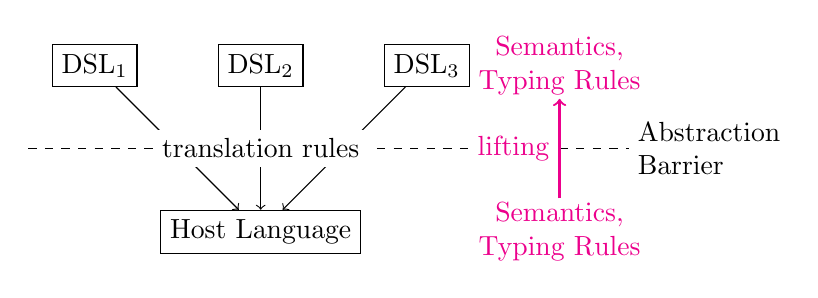
\begin{tikzpicture}[x=6pt,y=6pt,yscale=1,xscale=1]

\draw[dashed] (-14,5) -- (23,5);
\node[align=left,fill=white] at (27,5) {Abstraction\\Barrier};

\node[draw] (H) at (0,0) {Host Language};
\node[draw] (D1) at (-10,10) {DSL$_1$};
\node[draw] (D2) at (0,10) {DSL$_2$};
\node[draw] (D3) at (10,10) {DSL$_3$};

% \node[align=left,text=magenta] (M1) at (14,0) {Semantics, Typing Rules\\of Host Language}; 
\node[align=center,text=magenta] (M1) at (18,0) {Semantics,\\ Typing Rules}; 
\node[align=center,text=magenta] (M2) at (18,10) {Semantics,\\ Typing Rules}; 
 
\draw[->] (D1) -> (H);
\draw[->] (D3) -> (H);
\draw[->] (D2) -> node[fill=white] {translation rules} (H);
% \draw[->,thick,magenta] (9,2) -> node[right=1em] {lifting} (15,8);
\draw[->,thick,magenta] (18,2) -> node[left,fill=white] {lifting} (18,8);

\end{tikzpicture}

  \caption{Language Lifting}
  \label{fig:layers}
\end{figure}

% To this end, we describe the evaluation rules of the host language through a \textit{meta-language}.
% And the derived rules of the DSL is presented through meta-language as well.
% As a first step, the static derivation of semantic and typing rules for DSLs is called language lifting.
% We follow the core ideas of inferring typing rules for syntactic sugars \cite{infer-types} and apply it to semantics.
% For example, in a host language with lambda abstraction and application, we can define $\<let>$ by translation rule:
% \[ e_1~\<and>~e_2 => \<if>~e_1~\<then>~e_2~\<else>~\<false>. \]
% The derivation of $\<and>$ is given in Fig. \ref{fig:and}.

The evaluation rule derivation of $\<let>$ is given in Fig. \ref{fig:let}.
In DSL, an expression with $\<let>$ evaluates to $v$ in DSL,
 iff the translated problem evaluates to $v$ in host language (Step 1).
Based on the evaluation rule of application, we can futher expand the premise (Step 2).
A lambda abstraction is always a value, with no premises (Step 3). 
% And the evaluation rule of lambda abstraction can be applied.
Hence, we can obtain the following evaluation rule for $\<let>$:
\[
  \inference{e_1 \Da v_1 & e_2[v_1/x] \Da v}{\<let>~x:t=e_1~\<in>~e_2 \Da v}
\]
Note that without lambda abstraction and application appearing in the premises,
 the evaluation rule of $\<let>$ is described directly.
We define \textit{abstraction} property as evaluation rules of DSL should be independent of the host language.
And the abstraction property holds.

\begin{figure}[t!]
  \[
    \inference[(Step 1) ]{%
      \inference[(Step 2) ]{%
        \inference[(Step 3)]{}{%
          λx:t.e_2 \Da λx:t.e_2}
        & e_1 \Da v_1
        & e_2[v_1/x] \Da v
      }
      {(λx:t.e_2)~e_1 \Da v}
    }
    {\<let>~x:t=e_1~\<in>~e_2 \Da v}
  \]
  \caption{Evaluation Rule Derivation of $\mathit{let}$}
  \label{fig:let}
\end{figure}

This approach is seemingly natural but we are facing some challenges:
(1) In most cases it is not possible to statically determine where the lambda abstraction is called,
 and thus it is not possible to statically evaluate the abstraction body part directly.
 When a lambda abstraction is used in a translation rule for DSL constructs definition,
 the evaluation of inner language construct is delayed until that lambda abstraction is called in the DSL.
 Therefore, lambda abstraction with host language constructs may lead to abstraction leakage.
(2) \todo{substitution}

% This approach is seemingly natural but we are facing three challenges:
% (1) Unlike typing rules, which can typically be stated by one single rule,
% many evaluation rules, such as $\<if>$, do not conform this property:
% \[ \inference{e_1\Da \<true>  & e_2\Da v_2}{\<if>~e_1~e_2~e_3\Da v_2} \quad 
%    \inference{e_1\Da \<false> & e_3\Da v_3}{\<if>~e_1~e_2~e_3\Da v_3} 
% \]
% This may lead to nondeterminacy when searching rules in derivation. % or exponential growth in the number of rules.
% (2) Most type rules are defined in a modular way,
% which means the type of an expression just depends on the types of subexpressions,
% but the semantics may be not.
% In particular, when using lambda calculus as the host language,
% lambda abstraction itself is a value,
% so that a translation rule defined by lambda abstraction is a value as well.
% This may ruin the abstraction. 
% For example, $\<if>$ always appears in the evaluation rule of $\<andf>$,
%  which cannot be reduced:
% \[ \<andf> => λx:\<bool>.~λy:\<bool>.~\<if>~x~\<then>~y~\<else>~\<false>. \]
% (3) Since the rules of application include substitution,
% we must specify the expansion behaviour for expressions with substitution in semantic derivation.

% To address challenge (1),
% we introduce a variant of Skeleton \cite{skeleton} as meta-language to describe evaluation and typing rules.
% As a requirement, each language construct has unique evaluation and typing rules,
%  in order to guarantee the determinacy of derivation.
To address challenge (1),
 we propose \textit{lambda lifting}, to reveal the behaviour of lambda abstraction.
To address challenge (2),
 we put substitution as a meta-function, and prove that substitution keeps abstraction property of semantic derivation.

Defining DSL by translation rules allow developers to specialize the DSL constructs on the host language,
 enabling vertical language extensions.
Based on semantics lifting, the abstraction of DSL can be maintained.
But sometimes DSL cannot be defined by translation rules in an existing host language.
To solve this problem, when the expressiveness of the host language is insufficient, 
 our framework provide meta-extensions (to introduce new vocabularies) and monad-extensions (to introduce side-effects) on the host language
 to extend language horizontally without changing original semantics.
DSL developers can specialize the language structure of the DSL based on this extended host language.

% In this paper, we propose a new framework for DSL design.
% We use simply-typed lambda-calculus (\STLC) as the host language for its elementariness and versatility.
% To face the various demand of language features and enhance the versatility of the framework,
%  we propose a general DSL implementation flow.
% Our framework provide meta-extensions (to introduce new vocabularies) and monad-extensions (to introduce side-effects) on the host language.
% Then, users can specify DSL constructs by translation rules on the new extended host language.
% The framework will derive the evaluation rules and typing rules for these new constructs automatically,
%  to make the DSL standalone.
% All these rules are described by the meta-language. % and those of DSLs are generated.
% Finally and naturally, our framework will generate interpreters for DSLs based on these meta-language rules.
Our main technical contributions can be summarized as follows:

\begin{itemize}
  % \item We design a meta-language to describe the evaluation rules and typing rules of a language structurally.
  %   % The meta-language can be extended in a modular way.
  %   We formalize the syntax and semantics of our meta-language (Section \ref{sec:meta}).
  %   And then, we define the host language \STLC{} using meta-language (Section \ref{sec:m-host}).
  \item We present a semantic lifting algorithm for DSL constructs defined by translation rules (Section \ref{sec:tr}).
    As major properties of algorithms, we give proofs of correctness and abstraction. 
    % For translation rules defined with lambda abstraction,
    %  we illustrate lambda lifting algorithm to maintain abstraction property.
    % Besides, evaluation rules with substitution will not break these properties.
  \item We propose a general DSL implementation flow, using \STLC{} as the host language:
    first introduce vocabularies by meta-extensions and new language features by monad extensions (Section \ref{sec:ex}),
    then define the DSL constructs by translation rules on the extended language.
    % For each step, we give a formal description with examples.
    % And two strict requirements will be applied to translation rules.
  % \item We present an algorithm to derive evaluation and typing rules for DSL constructs defined by translation rules (Section \ref{sec:alg}).
  %   As major properties of algorithms, we give proofs of correctness and abstraction. 
  %   For translation rules defined with lambda abstraction,
  %    we illustrate lambda lifting method to maintain abstraction property.
  %   Besides, these properties can be guaranteed with substitution in derivation.
  \item We give an implementation of the framework called Osazone (Section \ref{sec:impl}).
    We use a nontrivial example with seven language implemented (three of them are designed as DSLs) as the evidence for the power of Osazone (Section \ref{sec:eval}).
\end{itemize}

% Note that the focus of this paper is on the semantics of the language rather than the syntax. 
% Extensions to the syntax, such as parser implementation for DSLs, are not the topic of this paper.
